\chapter{Continuity and Uniform Continuity}

A program samples $f(x)=1/x$ on a grid of points spaced $10^{-4}$ inside
$(0,1]$. Near $x=10^{-4}$ two neighboring points, namely $10^{-4}$ and
$2\times 10^{-4}$, give outputs $10000$ and $5000$; the difference is $5000$. Near
$x=1$ two neighboring points give $1$ and $1.0001$; the difference is about $10^{-4}$.
The same function, the same grid spacing, two differences seven powers apart.

The question that arises is not ``is $1/x$ continuous'', since the answer is yes at
every point of $(0,1]$. The question is a different one: how much grid spacing must be
used so that \emph{every} output on that interval stays inside a single tolerance? For
tolerance $10^{-2}$, the point $x=1$ demands only a spacing below
$9.901\times 10^{-3}$, whereas the point $x=10^{-4}$ demands a spacing below
$1.000\times 10^{-10}$. The ratio of the two demands is $9.9\times 10^{7}$. No single
spacing serves both, and that is not a defect of the program.

Chapter 4 supplied the limit of a sequence, Chapter 3 supplied the supremum, and neither
is enough: the limit of a function compares $f$ with one fixed number, so it cannot
compare two outputs from two nearby inputs. What is needed is one threshold for the
whole set, together with a way to prove that the threshold exists. This chapter builds
that tool, from the $\varepsilon$-$\delta$ definition to compact sets and the class of
Lipschitz functions, then closes with a function that is continuous at one point only.

\begin{untukanak}
Imagine a fire escape whose steps grow taller toward the top. At the bottom, one stride
the width of a foot raises us a little. At the top, the same stride raises us a hand's
width, then a forearm, then almost the height of a body. Our older sibling stands beside
us and asks one thing: how wide is a safe stride for the whole staircase? The honest
answer for a staircase like that does not exist. The width that is safe below is too
wide above, and the width that is safe above makes us crawl below.

Now the question that makes one curious. Is every staircase like that? There are
staircases whose steps are constant, and staircases whose steps change but never pass a
certain bound. For the second kind, one step width works from bottom to top. The
difference is not in the height of the staircase, but in how steeply its slope changes.

The same thing happens with the graph of a function. There are graphs that can be
controlled by one distance rule over their whole domain, and graphs that demand a
different rule at every point. In this chapter we will know why that difference can be
proved with certainty, and why a domain that is closed and bounded always belongs to the
first kind.
\end{untukanak}

\section{Limits of functions and the delta threshold}
\tingkat{basic}

The word ``approaches'' cannot be used as a definition, because everyone may mean
something different by it. What can be used is a wager: however much precision is
demanded, the output will fall inside that precision as long as the input is close
enough. In everyday language: we install a narrow window around $L$, and demand that $f$
enter that window for all $x$ close enough to $c$.

\kamus{functional limit}{limit fungsi}{a promise that the output can be forced into a
narrow window as long as the input is close enough to the door}

Before the definition, one technical term is needed. The point $c$ is called a
\emph{limit point}\index{limit point} of a set $A$ if every open interval around $c$
contains a point of $A$ other than $c$. Without that condition, the definition of limit
becomes vacuous at an isolated point.

\begin{definisi}[Limit of a function]
\index{limit of a function}
Let $A\subseteq\mathbb{R}$, $c$ a limit point of $A$, and $f\colon A\to\mathbb{R}$.
We write $\lim_{x\to c}f(x)=L$ if for every $\varepsilon>0$ there exists
$\delta>0$ such that for every $x\in A$ with $0<|x-c|<\delta$ we have
$|f(x)-L|<\varepsilon$.
\end{definisi}

Two things are easily missed. First, the condition $0<|x-c|$ means the value of $f$ at
$c$ is not counted; the function may be undefined at $c$ and the limit still exists.
Second, the order of the quantifiers: $\delta$ may depend on $\varepsilon$, but not on
$x$. In the section on uniform continuity, it is precisely that freedom which is at
issue.

This definition is a checking tool, not a recipe for finding $\delta$; $\delta$ is found
by working backward from $|f(x)-L|$. For
\[
f(x)=\frac{x^{2}-1}{x-1}\quad (x\neq 1),\qquad L=2,
\]
algebra gives $f(x)=x+1$, hence $|f(x)-2|=|x-1|$. So $\delta=\varepsilon$
works. For $\varepsilon=10^{-2}$ take $\delta=10^{-2}$: at $x=1+10^{-2}$ the
difference is exactly $10^{-2}$, and that does \emph{not} meet the strict condition; at
$x=1+5\times10^{-3}$ the difference is $5\times10^{-3}$. Therefore $\delta=\varepsilon/2$ is the safe
choice, and $\delta=\varepsilon$ is the cheapest choice whose bound is never
attained from inside.

One thing that may reasonably be demanded of a limit is its uniqueness: a function cannot
stop at two different places at once.

\begin{teorema}[Uniqueness of the limit]
\index{limit of a function}
If $\lim_{x\to c}f(x)=L_{1}$ and $\lim_{x\to c}f(x)=L_{2}$, then $L_{1}=L_{2}$.
\end{teorema}

\begin{proof}
Suppose $L_{1}\neq L_{2}$ and set $\varepsilon=|L_{1}-L_{2}|/2>0$. There is
$\delta_{1}>0$ such that $0<|x-c|<\delta_{1}$ gives $|f(x)-L_{1}|<\varepsilon$, and
there is $\delta_{2}>0$ such that $0<|x-c|<\delta_{2}$ gives $|f(x)-L_{2}|<\varepsilon$.
Take $x$ with $0<|x-c|<\min(\delta_{1},\delta_{2})$; such a point exists because
$c$ is a limit point. Then
\[
|L_{1}-L_{2}|\le|L_{1}-f(x)|+|f(x)-L_{2}|<2\varepsilon=|L_{1}-L_{2}|,
\]
an impossibility. Hence $L_{1}=L_{2}$.
\end{proof}

We also use one bridge that is not proved here: the limit of a function exists and
equals $L$ exactly when every sequence $x_{n}\to c$ with $x_{n}\neq c$ satisfies
$f(x_{n})\to L$. Its name is the sequence criterion; its proof is in Abbott,
\emph{Understanding Analysis}, Chapter 4, section Functional Limits, and in Rudin,
\emph{Principles of Mathematical Analysis}, Chapter 4, section Continuous Functions.
That bridge is what allows the sequences of Chapter 4 to be used for dismantling limits
that do not exist. For $g(x)=x/|x|$, the sequence $1/n$ gives $g\to 1$ while $-1/n$ gives
$g\to -1$; two different limits, so $\lim_{x\to 0}g(x)$ does not exist. That pattern is
used again for uniform continuity, with two sequences whose distance tends to zero.

\section{Continuity and its algebraic properties}
\tingkat{intermediate}

A limit compares $f$ with a number $L$ that stands on its own. Continuity asks for
something stricter: that number must be the value of the function at its point. In
everyday language: the graph does not jump at that point, and its value there really is
the value approached from the left and from the right.

\kamus{continuous}{kontinu}{a graph that can be drawn without lifting the pen at that
point}

\begin{definisi}[Continuity at a single point]
\index{continuous}
Let $f\colon A\to\mathbb{R}$ and $c\in A$. The function $f$ is \emph{continuous at $c$}
if for every $\varepsilon>0$ there exists $\delta>0$ such that for every $x\in A$
with $|x-c|<\delta$ we have $|f(x)-f(c)|<\varepsilon$. The function is called continuous
on $A$ if it is continuous at every point of $A$.
\end{definisi}

Note that $x=c$ is now allowed, and what is demanded is not merely that the limit exists,
but that the limit equals the value of the function. Continuity is therefore local: it
speaks only about the behavior of $f$ around one point.

For $f(x)=x^{2}$ at $c=2$ and $\varepsilon>0$ we have $|x^{2}-4|=|x-2|\,|x+2|$, and
if $|x-2|<1$ then $|x+2|<5$. So $\delta=\min(1,\varepsilon/5)$ works, whereas the
largest $\delta$ that is still valid is the positive root of $\delta(4+\delta)=\varepsilon$,
namely $2.49984376953\times10^{-4}$ for $\varepsilon=10^{-3}$. The gap between the two numbers
is the price of safety paid for not wanting to compute a root.
Figure~\ref{fig:epsdelta} shows the two thresholds for $\varepsilon=1$.

\begin{figure}[htbp]
\centering
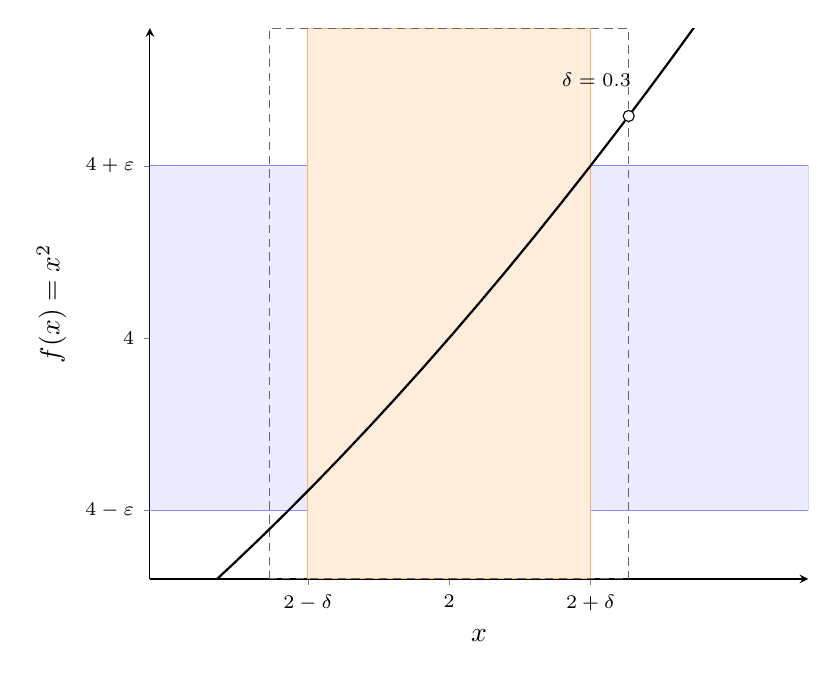
\begin{tikzpicture}
\begin{axis}[width=0.82\linewidth,
  axis lines=left,xmin=1.5,xmax=2.6,ymin=2.6,ymax=5.8,
  xlabel={$x$},ylabel={$f(x)=x^{2}$},
  xtick={1.7639,2,2.2361},xticklabels={$2-\delta$,$2$,$2+\delta$},
  ytick={3,4,5},yticklabels={$4-\varepsilon$,$4$,$4+\varepsilon$},
  tick label style={font=\scriptsize}]
\fill[blue!8,draw=blue!45] (1.5,3) rectangle (2.6,5);
\fill[orange!14,draw=orange!60] (1.7639,2.6) rectangle (2.2361,5.8);
\draw[densely dashed,black!60] (1.7,2.6) rectangle (2.3,5.8);
\addplot[thick,domain=1.5:2.6] {x^2};
\draw[fill=white] (2.3,5.29) circle (2pt);
\node[font=\scriptsize,anchor=east] at (2.32,5.5) {$\delta=0.3$};
\end{axis}
\end{tikzpicture}
\caption{The $\varepsilon$ band and the $\delta$ band for $f(x)=x^{2}$ at $a=2$ with
$\varepsilon=1$. The $\delta$ bound uses the formula $\delta=\sqrt{4+\varepsilon}-2$
in this section, so $\delta=\sqrt{5}-2\approx0.236$; the dashed band uses
$\delta=0.3$, and at $x=2.3$ the value $f(2.3)=5.29$ has already left the band.}
\label{fig:epsdelta}
\end{figure}

\begin{proposisi}
\index{continuous}
Let $c$ be a limit point of $A$. The function $f$ is continuous at $c$ if and only if
$\lim_{x\to c}f(x)=f(c)$.
\end{proposisi}

\begin{proof}
If $f$ is continuous at $c$ and $\varepsilon>0$, take $\delta$ from the definition of
continuity. For $0<|x-c|<\delta$ we have $|f(x)-f(c)|<\varepsilon$, and that is exactly
the definition of limit with $L=f(c)$. Conversely, if the limit is $f(c)$, take $\delta$
from the definition of limit; the condition $0<|x-c|$ can be dropped because for $x=c$
the inequality becomes $0<\varepsilon$, which is true.
\end{proof}

Continuity is closed under the operations usually used. In everyday language: adding,
multiplying, and dividing functions that do not jump produces functions that also do not
jump, as long as the divisor is not zero.

\begin{proposisi}[Algebraic properties and composition]
\index{continuous}
If $f$ and $g$ are continuous at $c$, then $f+g$, $fg$, and $cf$ are continuous at $c$;
if $g(c)\neq 0$, then $f/g$ is also continuous at $c$. If $f$ is continuous at $c$ and
$g$ is continuous at $f(c)$, then $g\circ f$ is continuous at $c$.
\end{proposisi}

\begin{proof}
The algebraic part follows the same limit rules as for sequences, with
$x_{n}\to c$ replaced by $x\to c$; since $c$ is a limit point, the sequence criterion
carries every statement about a limit of a function over to a statement about a limit of
a sequence, and the algebraic rules for sequences were proved in Chapter 4. For
composition, take $\varepsilon>0$. Since $g$ is continuous at $f(c)$, there is
$\eta>0$ such that $|y-f(c)|<\eta$ implies $|g(y)-g(f(c))|<\varepsilon$. Since $f$ is
continuous at $c$, for that $\eta$ there is $\delta>0$ such that $|x-c|<\delta$ implies
$|f(x)-f(c)|<\eta$. That chain of implications gives $|g(f(x))-g(f(c))|<\varepsilon$
whenever $|x-c|<\delta$.
\end{proof}

The pattern of the composition proof is worth remembering: two $\varepsilon$'s are used
in succession, and $\eta$ plays the role of $\varepsilon$ for the inner function. As a
consequence, polynomials and rational functions are continuous on their whole domain.
What is not guaranteed is a function defined by cases, and from there counterexamples
appear at the end of the chapter.

The crudest form of failure is a jump. The function in
Figure~\ref{fig:lompat} equals $x$ to the left of $1$, equals $2$ at the point $1$,
and equals $x+1$ to its right. At $x=1$ its value is $2$, whereas the values from the
left approach $1$. That difference of $1$ cannot be closed by any $\delta$, however small,
because for every $\delta$ there is still a point on the left with $|f(x)-f(1)|$ close
to $1$.

\begin{figure}[htbp]
\centering
\begin{tikzpicture}
\begin{axis}[width=0.70\linewidth,height=5.0cm,
  axis lines=left,xmin=0,xmax=2.2,ymin=0,ymax=3.2,
  xlabel={$x$},ylabel={$f(x)$},xtick={1},xticklabels={$1$},
  ytick={1,2,3},tick label style={font=\scriptsize},
  label style={font=\scriptsize}]
\fill[layerplum!12,draw=layerplum!60] (0,1.5) rectangle (2.2,2.5);
\addplot[densely dashed,layerplum] coordinates {(0.9,0) (0.9,3.2)};
\addplot[densely dashed,layerplum] coordinates {(1.1,0) (1.1,3.2)};
\addplot[thick,ink,domain=0:1,samples=2] {x};
\addplot[thick,ink,domain=1:2.2,samples=2] {x+1};
\addplot[only marks,mark=*,mark size=1.6pt,accent] coordinates {(0.95,0.95)};
\addplot[only marks,mark=o,mark size=2.6pt,ink,mark options={fill=white,solid}]
  coordinates {(1,1)};
\addplot[only marks,mark=*,mark size=1.7pt,ink] coordinates {(1,2)};
\draw[accent,->,>=stealth,thin] (0.60,1.30) -- (0.93,0.99);
\node[font=\scriptsize,layerplum,anchor=west] at (1.13,2.75) {$\delta$};
\node[font=\scriptsize,accent,anchor=west] at (0.10,1.22) {$f(0.95)=0.95$};
\node[font=\scriptsize,ink,anchor=north east] at (1.02,1.88) {$f(1)=2$};
\end{axis}
\end{tikzpicture}
\caption{A jump at $x=1$: $f(x)=x$ for $x<1$, $f(1)=2$, $f(x)=x+1$ for $x>1$.
The band $\varepsilon=\tfrac12$ around $f(1)=2$ is the horizontal strip between $1.5$ and
$2.5$, while the two dashed lines mark $|x-1|<0.1$. The point $x=0.95$ is already
inside that $\delta$ band, but its value $0.95$ is still $0.55$ below the lower edge of
the $\varepsilon$ band. The empty circle at $(1,1)$ is the value approached from the left,
not the value of the function. Shrinking $\delta$ does not help: a point on the left
closer to $1$ gives a value closer to $1$, not to $2$.}
\label{fig:lompat}
\end{figure}

\section{The intermediate value theorem}
\tingkat{intermediate}

In everyday language: to move from the lower room to the upper room, a climber has to
pass through every height in between. The graph of a continuous function cannot jump over
a value.

\begin{teorema}[Intermediate value]
\index{intermediate value theorem}
Let $f$ be continuous on $[a,b]$ and $f(a)<0<f(b)$. Then there is $c\in(a,b)$ with
$f(c)=0$. More generally, for every $v$ between $f(a)$ and $f(b)$ there is $c\in[a,b]$
with $f(c)=v$.
\end{teorema}

\begin{proof}
It is enough to prove the case $f(a)<0<f(b)$, because the general case is obtained by
applying that theorem to $f-v$. Form $S=\{x\in[a,b] : f(x)<0\}$. That set is not empty
because $a\in S$ and it is bounded above by $b$, so by the supremum property of Chapter 3,
$c=\sup S$ exists and $a\le c\le b$.

First, $f(c)\le 0$. Since $c$ is a supremum, there is a sequence $x_{n}\in S$ with
$x_{n}\to c$, and $f(x_{n})<0$ for every $n$. Continuity gives $f(x_{n})\to f(c)$, and a
limit preserves weak inequalities, so $f(c)\le 0$.

Second, $f(c)\ge 0$. Suppose $f(c)<0$. Since $f(b)>0$, the point $c$ is not $b$, so
$c<b$. Continuity at $c$ gives $\delta>0$ such that $|x-c|<\delta$ implies
$|f(x)-f(c)|<-f(c)$, in particular $f(x)<0$. For $\delta<2(b-c)$ the point $c+\delta/2$
lies in $[a,b]$ and satisfies $f(c+\delta/2)<0$, so it is a member of $S$; yet
$c+\delta/2>c=\sup S$. That impossibility gives $f(c)\ge 0$.

The two inequalities together give $f(c)=0$, and since $f(a)<0<f(b)$, that point lies in
$(a,b)$.
\end{proof}

Note that the proof gives no way of finding $c$. It only shows that the set of negative
points has a roof, and that the roof must be a root. The gap between ``exists'' and
``can be computed'' is what makes the intermediate value theorem used as a guarantee of
existence, not as an algorithm.

\begin{untukanak}
A climber starts in a valley and stops at a summit. They may rest, may walk backward for
a while, may stand still for a long time. What they do not do is jump. Therefore, if
there is a river in the valley and no river at the summit, there must be one point on
that path where they are for the first time exactly at the height of the river.

What makes one curious: how many such points are there? There may be one, there may be
three, there may be infinitely many, and the climber's story does not say which. It only
guarantees at least one. Mathematicians use that guarantee for something else: to prove
that an equation certainly has an answer, even though the answer cannot always be written
with a simple formula.

The next question is harder. What if the path is not connected, for example if there is a
chasm in the middle? The guarantee vanishes at once, and that is no prank: there are
functions whose value jumps from negative to positive without ever touching zero.
In this chapter we will know why the property ``does not jump'' is already enough, and
why that property has to be stated first before the theorem is used.
\end{untukanak}

Two immediate consequences are worth recording. First, the image of an interval under a
continuous function is an interval: $f([a,b])$ contains every value between $f(a)$ and
$f(b)$. Second, every continuous function $f\colon[0,1]\to[0,1]$ has a fixed point.
Consider $h(x)=f(x)-x$; at $x=0$ we have $h(0)=f(0)\ge 0$ and at $x=1$ we have
$h(1)=f(1)-1\le 0$. If either value is zero, that point is a fixed point. If not, the
intermediate value theorem gives $c$ with $h(c)=0$, that is $f(c)=c$.

The numbers in a concrete case can be checked. The equation $x^{3}+x-1=0$ has a root in
$(0,1)$ because $f(0)=-1<0<1=f(1)$. After twenty-one bisections, the root is trapped
between $0.682327747$ and $0.682328224$, with interval width $2^{-21}=4.768\times10^{-7}$;
the true value is $0.6823278038280193$. Bisection is not a proof, but the numbers can be
compared with the theoretical bound.

\section{The extreme value theorem}
\tingkat{intermediate}

In everyday language: on a road that is closed and unbroken, there is certainly a highest
point and a lowest point. Before proving it, we need one control: such a function cannot
run off to infinity.

\begin{lemma}
\index{extreme value theorem}
If $f$ is continuous on $[a,b]$, then $f$ is bounded on $[a,b]$.
\end{lemma}

\begin{proof}
Suppose $f$ is unbounded. Then for every $n$ there is $x_{n}\in[a,b]$ with
$|f(x_{n})|>n$. The sequence $(x_{n})$ is bounded, so by the
Bolzano--Weierstrass theorem of Chapter 4 there is a subsequence $x_{n_{k}}\to x$. Since
$a\le x_{n_{k}}\le b$ for all $k$, a limit preserves inequalities and
$x\in[a,b]$. Continuity at $x$ gives $f(x_{n_{k}})\to f(x)$, so that sequence is
bounded. Yet $|f(x_{n_{k}})|>n_{k}\to\infty$. That impossibility closes the
supposition.
\end{proof}

Now the main statement.

\begin{teorema}[Extreme value]
\index{extreme value theorem}
If $f$ is continuous on $[a,b]$, then there are $c,d\in[a,b]$ such that
$f(c)=\sup f([a,b])$ and $f(d)=\inf f([a,b])$. In other words, $f$ attains its
maximum and its minimum.
\end{teorema}

\begin{proof}
By the lemma, the set $f([a,b])$ is bounded and not empty, so $M=\sup f([a,b])$
exists and is finite. For every $n$ there is $x_{n}\in[a,b]$ with $f(x_{n})>M-1/n$;
such a sequence exists because $M$ is the least upper bound. By
Bolzano--Weierstrass there is a subsequence $x_{n_{k}}\to c$, and since
$a\le x_{n_{k}}\le b$ we get $c\in[a,b]$. Continuity at $c$ gives
$f(x_{n_{k}})\to f(c)$, while the trapping above gives $f(x_{n_{k}})\to M$.
Uniqueness of the limit gives $f(c)=M$. For the minimum, apply that result to $-f$.
\end{proof}

Both proofs use the same bridge: a bounded sequence inside a closed interval has a
subsequence that tends to a point inside that interval. Closedness is what ensures the
limit does not escape, and that is what is lost on an open interval.

The counterexample is simple. The function $f(x)=x$ is continuous on $(0,1)$ but attains
neither a maximum nor a minimum, because $0$ and $1$ are not members of its domain. The
function $g(x)=1/x$ is continuous on $(0,1]$ but unbounded there: $g(1/n)=n$. So
closedness and boundedness of the domain are not decoration; they are the entire reason
the theorem works.

As a consequence, for $f$ continuous on $[a,b]$ with $m=\inf f$ and $M=\sup f$, we have
$f([a,b])=[m,M]$. That equality combines two theorems: the first says $m$
and $M$ are attained, the second says all values in between are used.

\section{Uniform continuity}
\tingkat{advanced}

In the definition of continuity, $\delta$ may depend on $\varepsilon$ \emph{and}
on the point $c$. For $f(x)=1/x$ on $(0,1]$, every point has its own $\delta$,
and that $\delta$ shrinks without bound as $c$ approaches zero. Locally
everything is fine, but there is never one $\delta$ for the whole interval, and that is
what the grid in the chapter opening needs.

\kamus{uniform continuity}{kekontinuan seragam}{one step width that works from the foot of
the staircase to its top, not a different width on every step}

\begin{definisi}[Uniform continuity]
\index{uniform continuity}
A function $f\colon A\to\mathbb{R}$ is called \emph{uniformly continuous} on $A$ if for
every $\varepsilon>0$ there exists $\delta>0$ such that for all $x,y\in A$ with
$|x-y|<\delta$ we have $|f(x)-f(y)|<\varepsilon$.
\end{definisi}

Compare the two orders of quantifiers side by side:
\[
\text{continuous: } \ \forall c\in A\ \forall\varepsilon>0\ \exists\delta>0\
\forall x\in A,
\qquad
\text{uniform: } \ \forall\varepsilon>0\ \exists\delta>0\ \forall x,y\in A .
\]
In the uniform version, $\delta$ appears before $x$ and $y$ are introduced, so it may
not exploit knowledge of any point. That is the whole content of the difference, and
because of it uniformity is always relative to the set $A$: the same function can be
uniform on one set and not on another.

\begin{bacakeras}
Read aloud, two voices taking turns.

\textbf{Voice one:} Close at one point. However narrow the window installed, as long as
the input is close enough, the output is inside the window.

\textbf{Voice two:} Close at all points. It is not a question of which door. One window
width is installed first, then demanded to hold in the whole corridor, from the first
door to the last.

\textbf{Voice one:} If the corridor narrows at the end, that width has to be cut again
and again.

\textbf{Voice two:} And the cutting must not stop at one number. Stopping means one width
for the whole corridor; shrinking forever means a promise in installments.

Repeat this line until it feels right on the tongue: \emph{one point close enough, all
points one width.}
\end{bacakeras}

The statement that uniformity is stronger than continuity is proved directly from its
definition: uniformity gives one $\delta$ for all pairs of points, and
continuity only asks for a $\delta$ for pairs one of whose members is a fixed
point.

\begin{proposisi}
\index{uniform continuity}
If $f$ is uniformly continuous on $A$, then $f$ is continuous at every point of $A$.
\end{proposisi}

\begin{proof}
Take $c\in A$ and $\varepsilon>0$. Since $f$ is uniformly continuous, there is $\delta>0$
such that $|x-y|<\delta$ implies $|f(x)-f(y)|<\varepsilon$ for all $x,y\in A$.
Choosing $y=c$, the condition $|x-c|<\delta$ gives $|f(x)-f(c)|<\varepsilon$. That is
exactly the definition of continuity at $c$.
\end{proof}

The second way, used repeatedly in the rest of this chapter, works by contraposition: if
$f$ fails to be continuous at some point, two sequences whose distance tends to zero can
be built so that their outputs stay apart, and that refutes uniformity. The proof for
$1/x$ below uses that pattern in full.

Now an example showing that uniformity depends on the domain, not on the formula of the
function.

\begin{proposisi}
\index{uniform continuity}
$f(x)=x^{2}$ is uniformly continuous on $[0,1]$, with $\delta=\varepsilon/2$.
\end{proposisi}

\begin{proof}
For $x,y\in[0,1]$ we have $|x+y|\le 2$, hence
\[
|x^{2}-y^{2}|=|x-y|\,|x+y|\le 2|x-y| .
\]
If $|x-y|<\varepsilon/2$, then $|x^{2}-y^{2}|<\varepsilon$.
\end{proof}

That uniformity does not depend on the two endpoints: on $(0,1)$ the same proof still
works, because the bound $|x+y|\le 2$ uses no endpoint at all. The number
$\varepsilon/2$ is safe but not the best. For $|x-y|=\delta$ the largest difference
occurs at the end of the interval and equals $\delta(2-\delta)$, so $\delta$ is valid
provided $\delta\le 1-\sqrt{1-\varepsilon}$. For $\varepsilon=10^{-2}$ that bound is
$5.012563\times10^{-3}$, and with $\delta=\varepsilon/2$ the largest difference is
$9.975\times10^{-3}$.

\begin{proposisi}
\index{uniform continuity}
$f(x)=x^{2}$ is not uniformly continuous on $\mathbb{R}$.
\end{proposisi}

\begin{proof}
Take $\varepsilon=1$. Suppose there is $\delta>0$ that works. Choose a natural number
$n>1/\delta$ and set $x_{n}=n$, $y_{n}=n+1/n$. Then $|x_{n}-y_{n}|=1/n<\delta$,
but
\[
|x_{n}^{2}-y_{n}^{2}|=\left|n^{2}-\left(n+\tfrac1n\right)^{2}\right|
=2+\frac{1}{n^{2}}>2>1=\varepsilon .
\]
So no $\delta$ works for $\varepsilon=1$.
\end{proof}

The number $2$ in that computation is the point: the difference of values does not
shrink, it approaches $2$, even though the difference of inputs tends to zero. What fails
is the rate of change of $x^{2}$, which grows without bound, not its continuity. With
$\delta=10^{-4}$ and the pair $x=10^{4}$, $y=10^{4}+5\times10^{-5}$, the difference of
outputs is $1.0000000149$; with $\delta=10^{-2}$ and $x=100$, the difference is
$1.000025$. That number barely moves when $\delta$ shrinks ten thousand
times, and it is precisely that immobility which proves the failure of uniformity.

An equally important example is $1/x$, because here pointwise continuity never fails.

\begin{proposisi}
\index{uniform continuity}
$f(x)=1/x$ is not uniformly continuous on $(0,1]$, but is uniformly continuous on
$[1,\infty)$ with $\delta=\varepsilon$.
\end{proposisi}

\begin{proof}[Proof of the first part, with two sequences]
Take $x_{n}=1/n$ and $y_{n}=1/(n+1)$. Then
\[
|x_{n}-y_{n}|=\frac{1}{n(n+1)}\longrightarrow 0,
\qquad\text{but}\qquad
\left|\frac{1}{x_{n}}-\frac{1}{y_{n}}\right|=|n-(n+1)|=1
\]
for every $n$. If $f$ were uniformly continuous, take $\delta$ for $\varepsilon=1$;
for large $n$ we have $|x_{n}-y_{n}|<\delta$, so the difference of outputs would have to
be less than $1$. That contradicts the result above.
\end{proof}

\begin{proof}[Proof of the second part]
For $x,y\ge 1$ we have $xy\ge 1$, hence
\[
\left|\frac{1}{x}-\frac{1}{y}\right|=\frac{|x-y|}{xy}\le|x-y| .
\]
So $\delta=\varepsilon$ works, and the uniformity comes from one fact only: the
product $xy$ is never smaller than $1$.
\end{proof}

The pattern is clear. On $[1,\infty)$ the denominator $xy$ is kept away from zero by the
lower bound of the domain; on $(0,1]$ that denominator can be made as small as we like,
and that is where uniformity is lost. Uniformity is a property of the pair of function and
set, not of the function alone: $1/x$ appears in both propositions with two different
answers.

The largest threshold $\delta(c)$ at each point shows the difference as a picture.
For $c\in(0,1]$ and $\varepsilon>0$, the condition $1/(c-\delta)-1/c\le\varepsilon$ is
equivalent to $\delta\le\varepsilon c^{2}/(1+\varepsilon c)$, so the largest threshold at $c$
is $\delta(c)=\varepsilon c^{2}/(1+\varepsilon c)$, and
Figure~\ref{fig:delta-mengecil} plots it together with one fixed value
$\delta=\varepsilon/2$ that works for $x^{2}$ on $[0,1]$. The first curve falls
along a straight line with slope two on the log-log scale, from $9.901\times10^{-3}$ at $c=1$
to $1.000\times10^{-10}$ at $c=10^{-4}$; the second line is horizontal. Uniformity on
$[0,1]$ therefore reads as a horizontal line, and its failure on $(0,1]$
as a curve that never touches the floor.

\begin{figure}[htbp]
\centering
\begin{tikzpicture}
\begin{axis}[width=0.80\linewidth,height=5.8cm,
  xmode=log,ymode=log,xmin=8e-5,xmax=1.4,ymin=8e-11,ymax=4e-2,
  xlabel={point $c$},ylabel={threshold $\delta(c)$},
  grid=major,grid style={black!10},
  tick label style={font=\scriptsize},label style={font=\scriptsize},
  legend style={font=\scriptsize,at={(0.97,0.03)},anchor=south east,
    draw=black!15,fill=white,fill opacity=0.9,text opacity=1,row sep=1pt}]
\addplot[thick,accent,domain=1e-4:1,samples=80] {1e-2*x^2/(1+1e-2*x)};
\addlegendentry{$1/x$ on $(0,1]$, $\varepsilon=10^{-2}$}
\addplot[thick,layerteal,densely dashed,domain=1e-4:1] {5e-3};
\addlegendentry{$x^{2}$ on $[0,1]$, $\delta=\varepsilon/2$}
\addplot[only marks,mark=*,mark size=1.6pt,accent]
  coordinates {(1,9.901e-3) (1e-2,9.999e-7) (1e-4,1.0e-10)};
\node[font=\scriptsize,accent,anchor=south west] at (1.15e-4,1.7e-10)
  {$1.000\times10^{-10}$};
\node[font=\scriptsize,accent,anchor=east] at (0.92,1.05e-2) {$9.901\times10^{-3}$};
\end{axis}
\end{tikzpicture}
\caption{The largest threshold $\delta$ at each point $c$ for $1/x$ on $(0,1]$ with
$\varepsilon=10^{-2}$, namely $\delta(c)=\varepsilon c^{2}/(1+\varepsilon c)$, on a
log-log scale. The value falls from $9.901\times10^{-3}$ at $c=1$ to
$9.999\times10^{-7}$ at $c=10^{-2}$ and $1.000\times10^{-10}$ at $c=10^{-4}$,
so the graph is a straight line with slope two. The dashed line
$\delta=5\times10^{-3}$ is the safe choice $\varepsilon/2$ from the proof for $x^{2}$
on $[0,1]$: one and the same number works on that whole interval.}
\label{fig:delta-mengecil}
\end{figure}

\begin{tangan}
Materials: a corridor two meters long, chalk or paper tape, and a ruler.

Mark the floor at the point $0$, then walk with a stride that is continually halved:
half a meter, a quarter of a meter, an eighth of a meter, and so on. Mark every
footfall. After six or seven steps, stop and look at the marks from the end of the
corridor.

What needs to be seen: the marks cluster near the end, and the remaining distance shrinks
without ever becoming zero. That rule never finishes the journey, although every step is
valid according to its own rule.

Repeat with another rule: a fixed stride of half a meter all the way to the end. The
journey is finished in four steps, and one rule holds from the first mark to the last.
That is the difference between a rule that shrinks forever and one rule for the whole
corridor.
\end{tangan}

\section{Compactness, Lipschitz, and the Heine--Cantor theorem}
\tingkat{advanced}

In everyday language: on a domain that is closed and does not stretch to infinity,
ordinary continuity is already enough to give one threshold for all points. To state it,
we need one term about the domain.

\kamus{compact}{kompak}{a box that is closed tight and does not stick out without end}

\begin{definisi}[Compact]
\index{compact}
A set $K\subseteq\mathbb{R}$ is called \emph{compact} if every family of open sets whose
union contains $K$ has a finite subfamily whose union also contains $K$.
\end{definisi}

That definition is not practical to use directly. What saves us is its equivalence with
two properties that are easy to check: for sets in $\mathbb{R}$, compact is equivalent to
closed and bounded. That equivalence is known as the Heine--Borel theorem; we skip its
proof, and it is in Rudin, \emph{Principles of Mathematical Analysis}, Chapter 2, section
Compact Sets.

\begin{teorema}[Heine--Cantor]
\index{heine-cantor}
If $f$ is continuous on a compact set $K$, then $f$ is uniformly continuous on $K$.
\end{teorema}

\begin{proof}
Suppose $f$ is not uniformly continuous. Then there is $\varepsilon>0$ such that for every $n$
there are $x_{n},y_{n}\in K$ with $|x_{n}-y_{n}|<1/n$ but
$|f(x_{n})-f(y_{n})|\ge\varepsilon$. Since $K$ is bounded, $(x_{n})$ is bounded, and
by Bolzano--Weierstrass there is a subsequence $x_{n_{k}}\to x$. Since $K$ is closed,
$x\in K$. From $|x_{n_{k}}-y_{n_{k}}|<1/n_{k}$ we get $y_{n_{k}}\to x$ as well, and
$y_{n_{k}}\in K$. Continuity of $f$ at $x$ gives $f(x_{n_{k}})\to f(x)$ and
$f(y_{n_{k}})\to f(x)$, so $|f(x_{n_{k}})-f(y_{n_{k}})|\to 0$. That contradicts
$|f(x_{n_{k}})-f(y_{n_{k}})|\ge\varepsilon$. So the supposition is false.
\end{proof}

That proof uses the two properties of compactness separately: boundedness to trigger
Bolzano--Weierstrass, and closedness to ensure the limit point is still inside
$K$. Both are needed. On $(0,1)$, the function $1/x$ is continuous but not uniform, and
its domain is not closed. On $\mathbb{R}$, the function $x^{2}$ is continuous but not
uniform, and its domain is not bounded.

The following class of functions gives a shortcut that is often faster than checking the
definition.

\begin{definisi}[Lipschitz]
\index{lipschitz}
A function $f\colon A\to\mathbb{R}$ is called \emph{Lipschitz} if there is a constant $L\ge 0$
such that $|f(x)-f(y)|\le L|x-y|$ for all $x,y\in A$.
\end{definisi}

\begin{proposisi}
\index{lipschitz}
If $f$ is Lipschitz on $A$, then $f$ is uniformly continuous on $A$.
\end{proposisi}

\begin{proof}
Take $\varepsilon>0$. If $L=0$, the function is constant and any choice of $\delta$ works.
If $L>0$, take $\delta=\varepsilon/L$. For $|x-y|<\delta$ we have
$|f(x)-f(y)|\le L|x-y|<\varepsilon$.
\end{proof}

The converse does not hold, and the example shows that uniformity is weaker than
Lipschitz. The function $f(x)=\sqrt{x}$ is continuous on $[0,1]$, hence uniformly
continuous by the Heine--Cantor theorem. But
\[
\frac{|\sqrt{x}-\sqrt{0}|}{|x-0|}=\frac{1}{\sqrt{x}}\longrightarrow\infty
\quad (x\to 0^{+}),
\]
so no $L$ satisfies the Lipschitz definition. Thus Lipschitz is a sufficient condition,
not a necessary one. Conversely $x^{2}$ on $[0,1]$ is Lipschitz with $L=2$
and $1/x$ on $[1,\infty)$ with $L=1$, exactly the numbers in the preceding proofs.

\begin{tantangan}
The two examples of failure of uniformity in this chapter, $x^{2}$ on $\mathbb{R}$ and
$1/x$ on $(0,1]$, are both unbounded on their domains. Find a function that is
\emph{bounded} on $(0,1)$, continuous at every point, but not uniformly continuous
there, then prove it.

Hint 1: failure does not require values that grow; values that oscillate are enough,
with an oscillation that gets denser as $x$ approaches the end of the interval.

Hint 2: try $f(x)=\sin(1/x)$ with $x_{n}=1/(2\pi n+\pi/2)$ and
$y_{n}=1/(2\pi n-\pi/2)$. The function values are $1$ and $-1$, while
$|x_{n}-y_{n}|=\pi/((2\pi n)^{2}-(\pi/2)^{2})$ tends to zero.

If you are stuck, go back to the section Uniform continuity, the proof for $1/x$ with two
sequences.
\end{tantangan}

\section{A function that is continuous at one point only}
\tingkat{advanced}

Continuity is not built into all functions; it can fail on a very large set of points. The
cheapest example is built from the density of the rationals in Chapter 2.

\begin{contoh}
\index{dirichlet function}
Define $f\colon\mathbb{R}\to\mathbb{R}$ by $f(x)=x$ if $x$ is rational and
$f(x)=0$ if $x$ is irrational. Then $f$ is continuous at $0$ and not continuous at any
other point.
\end{contoh}

\begin{proof}
At $x=0$ we have $|f(x)-f(0)|=|f(x)|\le|x|$, because $f(x)$ always equals either $x$ or
$0$. So $\delta=\varepsilon$ works and $f$ is continuous at $0$.

Now take $c\neq 0$. Since $\mathbb{Q}$ and $\mathbb{R}\setminus\mathbb{Q}$
are both dense, there is a rational sequence $r_{n}\to c$ and an irrational sequence
$s_{n}\to c$. Then $f(r_{n})=r_{n}\to c$ while $f(s_{n})=0\to 0$. Two sequence limits
differ, so by the sequence criterion $\lim_{x\to c}f(x)$ does not exist, and $f$ is not
continuous at $c$.
\end{proof}

A close relative of that example is the indicator of the rationals, which equals $1$ at
rationals and $0$ at irrationals; that function is continuous at no point at all. The next
example is more interesting, because its set of continuity points is in fact large; it is
known as a modification of the Dirichlet function.

\begin{contoh}[Thomae's function, a Dirichlet modification]
\index{thomae function}
Define $t\colon[0,1]\to\mathbb{R}$ by $t(x)=0$ if $x$ is irrational, and
$t(x)=1/q$ if $x=p/q$ in lowest terms with $q\ge 1$. Then $t$ is
continuous at every irrational point and not continuous at every rational point.
\end{contoh}

\begin{proof}
Take $a$ irrational and $\varepsilon>0$. Choose $N$ with $1/N<\varepsilon$. The rational
numbers in $[0,1]$ with denominator $q\le N$ are finite in number, so among them there is
one closest to $a$; call its distance $\eta>0$. Since $a$ is irrational, that distance is
not zero. For $|x-a|<\eta$ there are two possibilities. If $x$ is irrational, then
$|t(x)-t(a)|=0<\varepsilon$. If $x=p/q$ with $q>N$, then
$|t(x)-t(a)|=1/q<1/N<\varepsilon$. So $t$ is continuous at $a$.

Now take $a=p/q$ rational. An irrational sequence $s_{n}\to a$ gives
$t(s_{n})=0\to 0$, while $t(a)=1/q>0$. The limit along that sequence is not equal to the
value of the function, so $t$ is not continuous at $a$.
\end{proof}

Both examples show that the set of discontinuity points can be the whole line, the set of
rationals, or a single point. The full classification, which states that this set is
always a countable union of closed sets, is in Rudin, Chapter 4, section
Discontinuities. Continuity that fails at many points is not an oddity but a structured
symptom.

\section{A worked example: a delta that depends on the point}
\tingkat{intermediate}

We return to $f(x)=x^{2}$ at $x_{0}=2$ with $\varepsilon=10^{-3}$, this time
down to the last digit.

\begin{resep}
Three steps for writing an $\varepsilon$-$\delta$ proof of $|f(x)-f(c)|<\varepsilon$:
\begin{enumerate}
  \item Work backward. Write $|f(x)-f(c)|$ as $|x-c|$ times a remainder, then find an
        upper bound for that remainder on the domain in use.
  \item Bound $|x-c|<1$ first (or $<r$) so that the remainder is bounded. Call
        its upper bound $M$, then set $\delta=\min(1,\varepsilon/M)$.
  \item Write the proof forward. Take $\varepsilon>0$, choose that $\delta$, suppose
        $|x-c|<\delta$, then derive $|f(x)-f(c)|<\varepsilon$ line by line.
\end{enumerate}
Steps 1 and 3 must not be swapped. The sentences of the proof are read from $\varepsilon$
to $\delta$, but $\delta$ is found in the opposite direction; writing directly from
$\varepsilon$ usually produces a $\delta$ that still contains $x$, and a choice like
that is not a valid $\delta$.
\end{resep}

The condition that must be satisfied is
\[
|x^{2}-4|=|x-2|\,|x+2|<\varepsilon
\]
for all $x$ with $|x-2|<\delta$. If $\delta<1$, then $|x+2|<4+\delta$,
so it is enough to demand $\delta(4+\delta)=\varepsilon$. That quadratic equation
has the positive root
\[
\delta=\sqrt{4+\varepsilon}-2 .
\]
For $\varepsilon=10^{-3}$ that formula gives $\delta=2.49984376953\times10^{-4}$.
A check at three points:
\[
\begin{array}{lll}
|x-2|=2.497343925761\times10^{-4} & \Rightarrow & |x^{2}-4|=9.989999375719\times10^{-4},\\
|x-2|=2.499843769530\times10^{-4} & \Rightarrow & |x^{2}-4|=1.000000000000\times10^{-3},\\
|x-2|=2.502343613300\times10^{-4} & \Rightarrow & |x^{2}-4|=1.001000062555\times10^{-3}.
\end{array}
\]
The second row shows that the largest $\delta$ produces a difference of exactly
$\varepsilon$; the third row, that going slightly past it already violates the condition.
The popular choice $\delta=\varepsilon/4=2.5\times10^{-4}$ turns out to \emph{fail}: the
difference is $1.0000625\times10^{-3}$, larger than $\varepsilon$ by $6.25\times10^{-8}$.
A failure that small is easily missed when checked with three-digit truncation.

Now notice how $\delta$ depends on the point. For
$\varepsilon=10^{-2}$ and $f(x)=x^{2}$, the positive root of $\delta(2x_{0}+\delta)=\varepsilon$
is $\delta=\sqrt{x_{0}^{2}+\varepsilon}-x_{0}$.

\begin{center}
\small
\begin{tabular}{rrrr}
\hline
$x_{0}$ & largest $\delta$ & $\delta/x_{0}$ & $\varepsilon/(2x_{0})$ \\
\hline
$1$ & $4.987562\times10^{-3}$ & $4.987562\times10^{-3}$ & $5.000000\times10^{-3}$ \\
$2$ & $2.498439\times10^{-3}$ & $1.249220\times10^{-3}$ & $2.500000\times10^{-3}$ \\
$10$ & $4.999875\times10^{-4}$ & $4.999875\times10^{-5}$ & $5.000000\times10^{-4}$ \\
$100$ & $4.999999\times10^{-5}$ & $4.999999\times10^{-7}$ & $5.000000\times10^{-5}$ \\
$1000$ & $5.000000\times10^{-6}$ & $5.000000\times10^{-9}$ & $5.000000\times10^{-6}$ \\
$10^{4}$ & $5.000002\times10^{-7}$ & $5.000002\times10^{-11}$ & $5.000000\times10^{-7}$ \\
\hline
\end{tabular}
\end{center}

The third column shrinks as fast as $1/x_{0}^{2}$, and for large $x_{0}$ the value of
$\delta$ is practically the same as $\varepsilon/(2x_{0})$. So there is no positive lower
bound for $\delta$ as $x_{0}$ grows: the rate of change of $x^{2}$ at $x_{0}$ is $2x_{0}$,
and that rate is what sets the threshold, not rounding.

The failure of uniformity of $x^{2}$ on $\mathbb{R}$ was proved in the section Uniform
continuity and is repeated by machine in the Computational lab, part 3, so the numbers are
not repeated here. What has not yet appeared as a picture is the dependence on the domain,
and that is shown by $1/x$. On $[1,\infty)$ with $\delta=\varepsilon$ the largest
difference occurs at $x=1$ and equals $\varepsilon/(1+\varepsilon)$, namely
$9.900990\times10^{-3}$ for $\varepsilon=10^{-2}$. On $(0,1]$ the pair $x=1/n$,
$y=1/(n+1)$ gives an output difference of exactly $1$ while the input distance shrinks:

\begin{center}
\small
\begin{tabular}{rrr}
\hline
$n$ & $|x-y|$ & $|1/x-1/y|$ \\
\hline
$10$ & $9.091\times10^{-3}$ & $1$ \\
$100$ & $9.901\times10^{-5}$ & $1$ \\
$1000$ & $9.990\times10^{-7}$ & $1$ \\
$10^{4}$ & $9.999\times10^{-9}$ & $1$ \\
\hline
\end{tabular}
\end{center}

\kertas{For $f(x)=x^{2}$ and $\varepsilon=10^{-2}$, compute the largest $\delta$ at
$x_{0}=1000$ from the formula $\sqrt{x_{0}^{2}+\varepsilon}-x_{0}$, then compare with
$\varepsilon/(2x_{0})$. Check that the difference at $x=x_{0}+\delta$ is exactly
$\varepsilon$, and explain why that formula cannot be used to prove uniformity on
$\mathbb{R}$.}

\section{Computational lab: measuring uniformity}
\tingkat{advanced}

The eight checks below turn the previous sections into numbers that can be rechecked:
explicit $\delta$ and its bound, its dependence on the point, $x^{2}$ and $1/x$ on two
domains, the largest threshold at each point, and bisection for the intermediate value
theorem.

\begin{lab}
\begin{verbatim}
import math

# 1. optimal delta for f(x)=x^2 at x0=2, eps=1e-3
def delta_sq(x0, eps):
    return math.sqrt(x0*x0 + eps) - x0

eps = 1e-3
d = delta_sq(2.0, eps)
print("== 1. explicit delta, x0=2, eps=1e-3 ==")
print("optimal delta = %.12f" % d)
for t in (d*0.999, d, d*1.001):
    print("  x-2=%.12e  |x^2-4|=%.12e" % (t, abs((2+t)**2-4)))
print("  delta=eps/4 -> |x^2-4|=%.12e" % abs((2+eps/4)**2-4))

# 2. delta depending on the point
print("== 2. delta(x0) for eps=1e-2 ==")
print("      x0       delta     delta/x0")
for x0 in (1.0, 2.0, 10.0, 100.0, 1000.0, 1e4):
    d = delta_sq(x0, 1e-2)
    print("%8.0f  %.6e  %.6e" % (x0, d, d/x0))

# 3. failure of uniformity of x^2 on R
print("== 3. x^2 on R, eps=1 ==")
print("   delta   x=1/delta   |x^2-(x+d/2)^2|")
for delta in (1e-1, 1e-2, 1e-3, 1e-4):
    x = 1.0/delta
    print("%8.0e %9.0f   %.10f" % (delta, x, abs(x*x-(x+delta/2)**2)))

# 4. x^2 on [0,1]
print("== 4. x^2 on [0,1], |x-y|=delta ==")
print("   delta    2d-d^2       grid")
for delta in (1e-1, 1e-2, 1e-3):
    n = int(round(1/delta))
    g = max(abs((i*delta/n)**2-(i*delta/n+delta)**2)
            for i in range(0, int(n*(1-delta)/delta)+1))
    print("%8.0e  %.10e %.10e" % (delta, 2*delta-delta*delta, g))

# 5. 1/x on [1,inf) and on (0,1]
print("== 5. 1/x on [1,inf), delta=eps ==")
for eps in (1e-1, 1e-2, 1e-3):
    s = max(abs(1/x-1/(x+eps)) for x in [1+i*eps/500 for i in range(501)])
    print("eps=%.0e  sup=%.10e  eps/(1+eps)=%.10e" % (eps, s, eps/(1+eps)))
print("== 6. 1/x on (0,1]: x=1/n, y=1/(n+1) ==")
print("      n      |x-y|      |1/x-1/y|")
for n in (10, 100, 1000, 10000):
    print("%7d   %.3e       %.1f" % (n, 1/n-1/(n+1), 1.0))

# 7. largest valid delta at c, f=1/x, eps=1e-2
print("== 7. delta(c) for 1/x, eps=1e-2 ==")
print("       c      delta(c)    delta/c")
for c in (1.0, 1e-1, 1e-2, 1e-3, 1e-4):
    dd = 1e-2*c*c/(1+1e-2*c)
    print("%8.0e  %.4e  %.4e" % (c, dd, dd/c))

# 8. numerical IVT for x^3+x-1=0
print("== 8. root of x^3+x-1=0 by bisection ==")
lo, hi = 0.0, 1.0
for k in range(1, 22):
    mid = (lo+hi)/2
    if mid**3+mid-1 < 0:
        lo = mid
    else:
        hi = mid
    if k in (1, 5, 10, 15, 20, 21):
        print("k=%2d  [%.12f, %.12f]  width=%.3e"
              % (k, lo, hi, hi-lo))
print("f(lo)=%.3e  f(hi)=%.3e" % (lo**3+lo-1, hi**3+hi-1))
\end{verbatim}
\end{lab}

\newpage
The output, as it stands:

\begin{verbatim}
== 1. explicit delta, x0=2, eps=1e-3 ==
optimal delta = 0.000249984377
  x-2=2.497343925761e-04  |x^2-4|=9.989999375719e-04
  x-2=2.499843769530e-04  |x^2-4|=1.000000000000e-03
  x-2=2.502343613300e-04  |x^2-4|=1.001000062555e-03
  delta=eps/4 -> |x^2-4|=1.000062499999e-03
== 2. delta(x0) for eps=1e-2 ==
      x0       delta     delta/x0
       1  4.987562e-03  4.987562e-03
       2  2.498439e-03  1.249220e-03
      10  4.999875e-04  4.999875e-05
     100  4.999999e-05  4.999999e-07
    1000  5.000000e-06  5.000000e-09
   10000  5.000002e-07  5.000002e-11
== 3. x^2 on R, eps=1 ==
   delta   x=1/delta   |x^2-(x+d/2)^2|
   1e-01        10   1.0025000000
   1e-02       100   1.0000250000
   1e-03      1000   1.0000002499
   1e-04     10000   1.0000000149
== 4. x^2 on [0,1], |x-y|=delta ==
   delta    2d-d^2       grid
   1e-01  1.9000000000e-01 1.9000000000e-01
   1e-02  1.9900000000e-02 1.9900000000e-02
   1e-03  1.9990000000e-03 1.9990000000e-03
== 5. 1/x on [1,inf), delta=eps ==
eps=1e-01  sup=9.0909090909e-02  eps/(1+eps)=9.0909090909e-02
eps=1e-02  sup=9.9009900990e-03  eps/(1+eps)=9.9009900990e-03
eps=1e-03  sup=9.9900099900e-04  eps/(1+eps)=9.9900099900e-04
== 6. 1/x on (0,1]: x=1/n, y=1/(n+1) ==
      n      |x-y|      |1/x-1/y|
     10   9.091e-03       1.0
    100   9.901e-05       1.0
   1000   9.990e-07       1.0
  10000   9.999e-09       1.0
== 7. delta(c) for 1/x, eps=1e-2 ==
       c      delta(c)    delta/c
   1e+00  9.9010e-03  9.9010e-03
   1e-01  9.9900e-05  9.9900e-04
   1e-02  9.9990e-07  9.9990e-05
   1e-03  9.9999e-09  9.9999e-06
   1e-04  1.0000e-10  1.0000e-06
== 8. root of x^3+x-1=0 by bisection ==
k= 1  [0.500000000000, 1.000000000000]  width=5.000e-01
k= 5  [0.656250000000, 0.687500000000]  width=3.125e-02
k=10  [0.681640625000, 0.682617187500]  width=9.766e-04
k=15  [0.682312011719, 0.682342529297]  width=3.052e-05
k=20  [0.682327270508, 0.682328224182]  width=9.537e-07
k=21  [0.682327747345, 0.682328224182]  width=4.768e-07
f(lo)=-1.354e-07  f(hi)=1.007e-06
\end{verbatim}

There are four things to read from that output, and all of them were predicted before the
program ran. Part 1 confirms that the optimal $\delta$ produces a difference of exactly
$10^{-3}$, whereas $\delta=\varepsilon/4$ produces $1.0000625\times10^{-3}$:
that popular choice does fail, not merely look untidy. Part 2 confirms that
the column $\delta/x_{0}$ falls as fast as $1/x_{0}^{2}$ up to $x_{0}=1000$, then stops
following the pattern at $x_{0}=10^{4}$. At the last point the true value is
$4.99999999987\times10^{-7}$, while float64 prints $5.000002\times10^{-7}$; that is
cancellation error in $\sqrt{x_{0}^{2}+\varepsilon}-x_{0}$, not a property of the function, and
that is why such a formula is not used at large scale.

Parts 3 through 7 show two faces of the same function. On $\mathbb{R}$ the difference
for $x^{2}$ stays above $1$ for every $\delta$ tried; on $[0,1]$ the largest
difference is $2\delta-\delta^{2}$, and the grid prints the same number to ten
digits because the largest difference occurs at $x=1-\delta$, a point that is in the grid
list. On $[1,\infty)$ the difference for $1/x$ is exactly $\varepsilon/(1+\varepsilon)$,
whereas on $(0,1]$ it stays $1.0$ while the input distance shrinks to
$9.999\times10^{-9}$. Part 8 closes with interval width $2^{-21}$ after twenty-one
bisections, and the root of $x^{3}+x-1$ is trapped inside it.

The program does not prove a single one of those things. It checks claims that have already
been proved, and in two places it shows the limits of itself: the failure of
$\delta=\varepsilon/4$ only becomes visible at the eighth digit, and cancellation error
only becomes visible at $x_{0}=10^{4}$.

\begin{untukdosen}
The teaching order I suggest: start from the grid in the chapter opening, not from the
definition. Write $10000$ and $5000$ on the board, ask what grid spacing is needed at
that point, then compare with the answer at $x=1$; from that gap the
$\varepsilon$-$\delta$ definition appears as the answer to a question that has already
been felt, not as a sentence to memorize. After that continuity, the algebraic properties,
the intermediate value theorem, the extreme value theorem, then uniform continuity and
Heine--Cantor.

Two misconceptions appear most often. First, students believe $\delta$ may depend on $x$
inside the definition of continuity, then ``prove'' uniformity by choosing a different
$\delta$ at every point; the symptom shows when they cannot name one $\delta$ for two
distant points. Second, they think the intermediate value theorem gives a way of
computing a root, whereas it only guarantees existence.

A blackboard activity that works: ask two students to play challenger and responder for
$f(x)=x^{2}$ at $x_{0}=2$ and at $x_{0}=1000$ with the same $\varepsilon$,
then have the class guess at which point the responder runs out of numbers. The sign that
the class is ready to move on: they can name one explicit $\delta$ for $1/x$
on $[1,\infty)$ and explain why the same $\delta$ fails on $(0,1]$.
\end{untukdosen}

\section{Summary}
\tingkat{basic}

\begin{ringkasan}
\begin{itemize}
  \item $\lim_{x\to c}f(x)=L$ means that for every $\varepsilon>0$ there is $\delta>0$
        such that $0<|x-c|<\delta$ gives $|f(x)-L|<\varepsilon$. The value at $c$
        itself is not counted, and the limit is unique.
  \item $f$ is continuous at $c$ if the limit exists and equals $f(c)$. Continuity
        is local, closed under algebraic operations, and preserved under
        composition.
  \item On a closed bounded interval, a continuous function is bounded, attains its
        maximum and minimum, and takes all values in between. All three can
        fail on an open interval.
  \item $f$ is uniformly continuous if one $\delta$ works for all pairs of points.
        Uniformity is stronger than continuity, and uniformity is always relative
        to its domain.
  \item $x^{2}$ is uniform on $[0,1]$ but not on $\mathbb{R}$; $1/x$ is uniform
        on $[1,\infty)$ but not on $(0,1]$. A function continuous on a compact
        set is always uniform, and a Lipschitz function is always uniform.
  \item Continuity can fail on a large set of points: the rational indicator fails
        everywhere, $x$ at rationals and $0$ at irrationals fails at every point
        except zero.
\end{itemize}
\end{ringkasan}

\section{Exercises}
\tingkat{intermediate}

\begin{latihan}
\begin{enumerate}
  \item Prove from the definition that $\lim_{x\to 3}(2x-1)=5$, and give the smallest
        explicit $\delta$ as a function of $\varepsilon$. Explain why
        $\delta=\varepsilon/2$ is the largest valid choice, whereas
        $\delta=\varepsilon/3$ is valid but smaller than necessary.
  \item Prove that $f(x)=x^{2}$ is continuous at every point $c\in\mathbb{R}$ with
        $\delta=\min(1,\varepsilon/(2|c|+1))$, then check that formula at $c=2$ and
        $c=100$ for $\varepsilon=10^{-2}$.
  \item Assess this claim: ``Because $1/x$ is continuous at every point of $(0,1]$, that
        function is uniformly continuous on $(0,1]$.'' True, false, or not enough
        evidence? Name the part that is correct and the part that is wrong.
  \item Prove that if $f$ and $g$ are uniformly continuous on $A$, then $f+g$ is uniformly
        continuous on $A$. Show by example that $fg$ need not be uniformly
        continuous on an unbounded $A$.
  \item Prove that $f(x)=\sqrt{x}$ is uniformly continuous on $[0,\infty)$ by
        using $|\sqrt{x}-\sqrt{y}|\le\sqrt{|x-y|}$. Explain why the proof does not
        require the domain to be closed.
  \item Compute the largest $\delta$ for $f(x)=x^{3}$ at $x_{0}=1$ with
        $\varepsilon=10^{-2}$ by solving $(1+\delta)^{3}-1=\varepsilon$, then
        compare with $\delta=\varepsilon/3$. Check both values in Python.
  \item For $f(x)=x^{2}$ on $[0,1]$ and $\varepsilon=10^{-2}$, compute the largest
        difference for $\delta=\varepsilon/2$ and for $\delta=1-\sqrt{1-\varepsilon}$.
        Show that the first choice is safe but not optimal, and that the second
        choice produces a difference of exactly $\varepsilon$.
  \item Prove that if $f$ is continuous on $[a,b]$ and $f(x)\neq 0$ for all
        $x\in[a,b]$, then there is $m>0$ with $|f(x)|\ge m$ for all $x$. Use the
        extreme value theorem, and explain why the conclusion fails for
        $f(x)=x$ on $(0,1)$.
  \item Define $f(x)=x$ if $x$ is rational and $f(x)=-x$ if $x$ is irrational.
        Prove that $f$ is continuous only at $0$, then show that $|f|$ is continuous at
        every point. Explain why the second result does not contradict the first.
\end{enumerate}

Hints for the three hardest items. Item 4: for the second part, take $f(x)=g(x)=x$
on $\mathbb{R}$ and use the pair $x_{n}=n$, $y_{n}=n+1/n$. Item 5: square
$|\sqrt{x}-\sqrt{y}|\le\sqrt{|x-y|}$ to see where it comes from. Item 9: $|f|$ is none
other than $x\mapsto|x|$, which is continuous everywhere; for $c\neq0$ use rational
and irrational sequences tending to $c$.
\end{latihan}

\begin{untukpeneliti}
What is proved in this chapter: uniformity is stronger than continuity; continuity
on a compact set gives uniformity; continuity on a closed bounded interval
gives boundedness, extreme values, and the intermediate value property. What is popular but
not proved is the impression that the intermediate value theorem gives an algorithm: it
only gives existence, and the rate $2^{-n}$ comes from the procedure, not from the
theorem.

Primary sources: Rudin, \emph{Principles of Mathematical Analysis}, Chapter 4, section
Continuity and Compactness, which proves Heine--Cantor in the framework of general metric
spaces; and Abbott, \emph{Understanding Analysis}, Chapter 4, sections Continuous Functions on
Compact Sets and Sets of Discontinuity. The proof of Heine--Borel is deliberately skipped
here and is in Rudin, Chapter 2, section Compact Sets.

Limit of validity: the whole chapter works in $\mathbb{R}$ with the usual distance. In a
metric space, the definition of uniformity stays the same word for word, but the
Heine--Cantor theorem demands compactness, not merely closedness and boundedness; in an
infinite-dimensional space those two properties separate. In a complete metric space,
uniformity on a dense set is enough to extend a function uniquely, and that is the door
into the extension theorems not discussed here.

A question still open for the reader: how fast the modulus of continuity
$\omega(\delta)=\sup_{|x-y|<\delta}|f(x)-f(y)|$ may fall. For a function continuous
on a closed interval, $\omega(\delta)\to 0$ is guaranteed, but the rate of its decrease is
not: there are continuous functions whose modulus falls more slowly than every power
$\delta^{\alpha}$. The Lipschitz guarantee that is often assumed on adversarial attack
bounds in Chapter 29 is therefore sufficient, not necessary.
\end{untukpeneliti}

\peta{Chapter 11 in Rudin, \emph{Principles of Mathematical Analysis}: Chapter 4 (Continuous
Functions, Continuity and Compactness, Continuity and Connectedness, Discontinuities),
with the Heine--Borel theorem taken from Chapter 2, section Compact Sets. In Abbott,
\emph{Understanding Analysis}: Chapter 4 (Discussion: Examples of Dirichlet and Thomae,
Functional Limits, Combinations of Continuous Functions, Continuous Functions on
Compact Sets, The Intermediate Value Theorem, Sets of Discontinuity). The
$\varepsilon$-$\delta$ definition and the sequence criterion are built from the sequences in Chapter 4 of this
book, whereas the supremum used to prove the intermediate value theorem comes from Chapter 3.
The derivative in Chapter 12 continues this chapter by using the difference quotient as a limit,
and Chapter 27 uses uniformity as one of the guarantees that is often assumed
without being checked.}
